\documentclass[a4paper,18pt]{article}
\usepackage{blindtext}
\usepackage[romanian]{babel}
\usepackage[utf8]{inputenc}
\usepackage{tabto}
\usepackage{graphicx}

\title{SUDOKU}
\begin{document}
\maketitle

\author{
\begin{center}
  \texttt{PELE CARMEN-IOANA}
  \and
\end{center}
\begin{center}
  \texttt{STAN ALEXANDRA-PAULA}
\end{center}
}

\begin{figure}[h!]
\begin{center}
  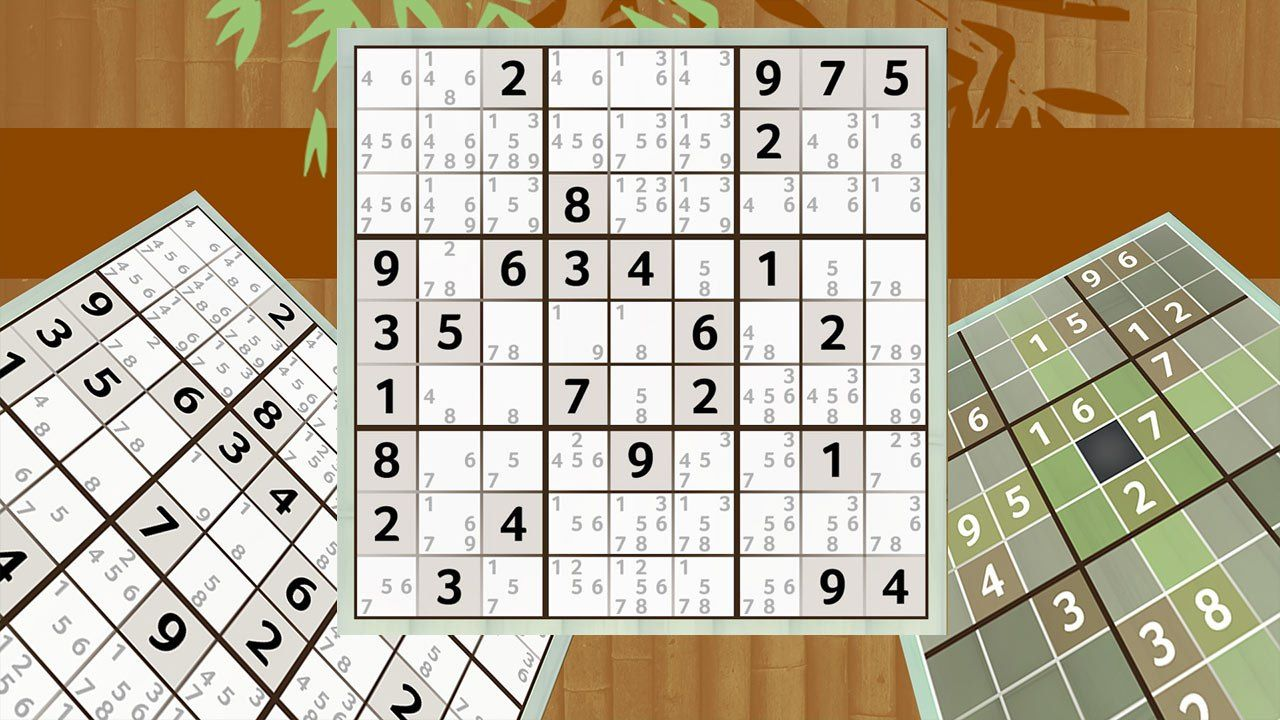
\includegraphics[width=0.8\linewidth]{sudoku.jpg}
\end{center}
\end{figure}

\renewcommand{\contentsname}{CUPRINS}
\vspace{16cm}
\tableofcontents
\vspace{14cm}
\section{ Introducere}

\tab Sudoku este un joc sub forma de grila, aparut prima data in anul 1979. A fost precedat si inspirat de patratul latin si problema celor 36 de ofiteri a lui Leonhard Euler. Descrierea jocului nefiind foarte ampla, trebuie completata grila cu numere de la 1 la 9. Cifrele reprezinta doar o conventie, acestea pot fi inlocuite cu ltere sau culori. 
\newline Situatia initiala este in doua variante:
\newline 
\\ \indent - grila este complet goala
\newline 
\\ \indent - grila contine cateva numere pentru a conditiona rezultatul final.
\newline 
\\ \indent Regula principala a jocului este completarea celulelor din regiuni (o regiune este formata din 3 x 3 celule) astfel incat pe linie si pe coloana sa nu fie doua cifre identice (conditia se aplica pentru toata grila (grila este formata din regiuni 3 x 3, ulterior formata din 9 x 9 celule). Cei trei pasi folositi pentru a rezolva un puzzle de tip Sudoku sunt: cautarea si verificarea cifrelor candidate.

\section{ Descrierea aplicatiei}

\tab Aplicatia intitulata Sudoku este impartita pe trei fisiere: "main.py", "sudoku.py", "util.py".

 In main se regaseeste ceea ce priveste interfata proiectata si arata in urmatorul mod:

\begin{figure}[h!]
\begin{center}
  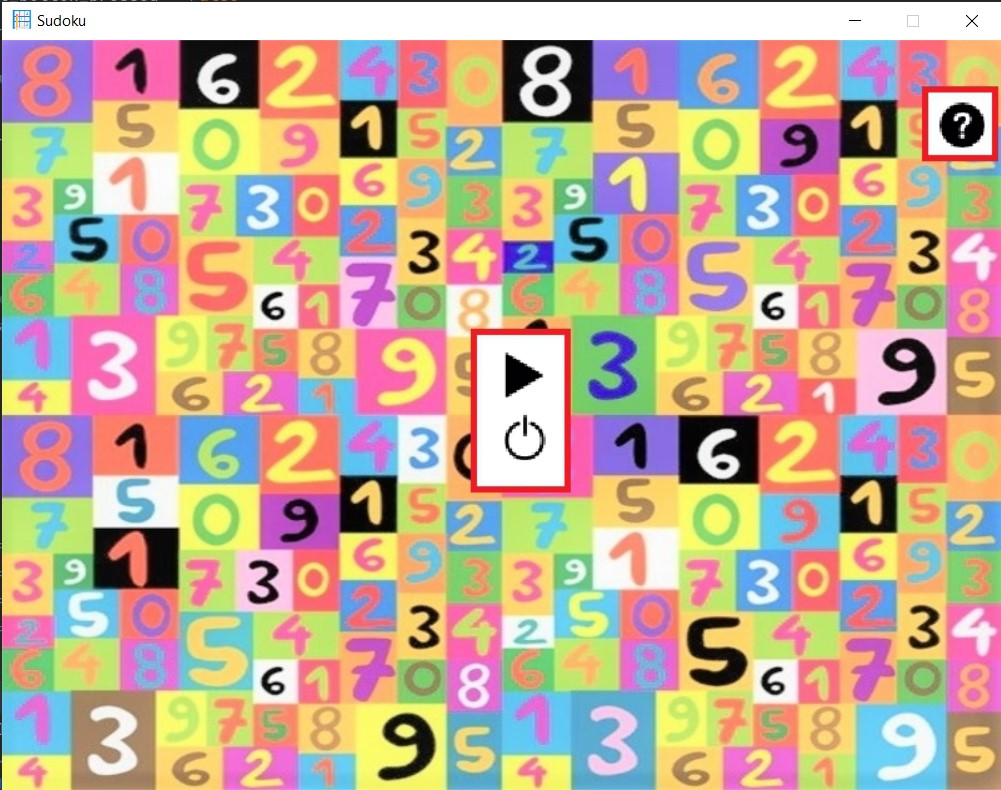
\includegraphics[width=0.8\linewidth]{1.jpg}
  \caption{Pagina de start}
  \label{fig:start}
\end{center}
\end{figure}

\newpage
Se regaseste in titlu numele jocului. Butoanele existente sunt cele de "Start" "Stop" si "Ajutor". 

\begin{figure}[h!]
  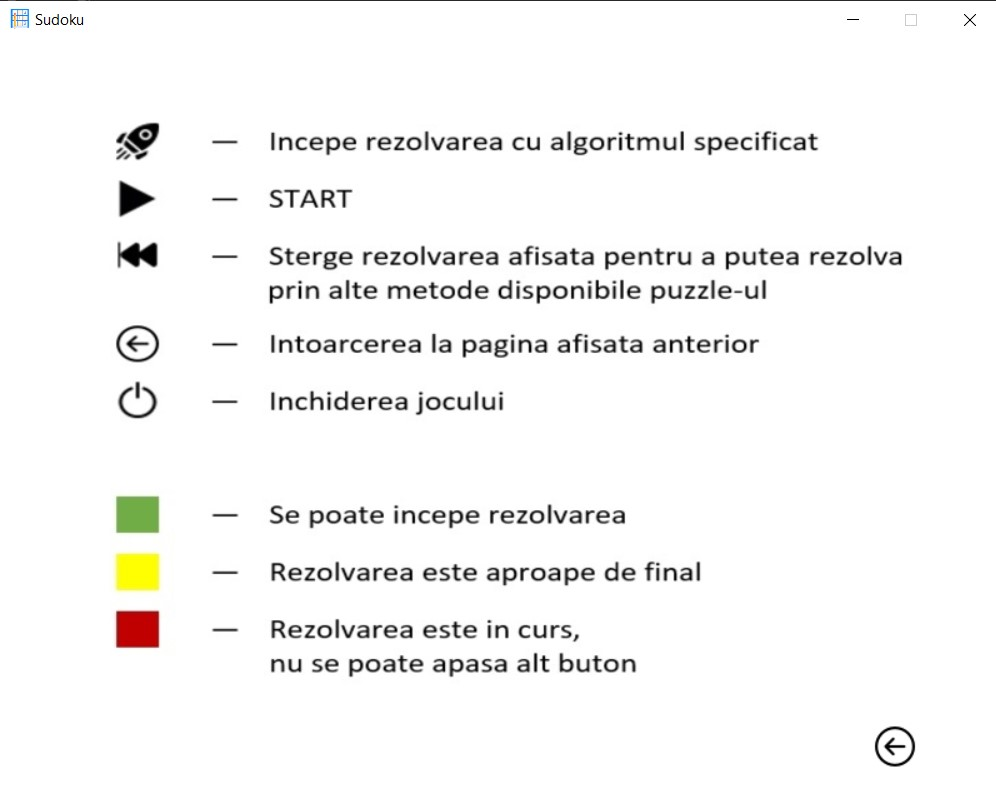
\includegraphics[width=\linewidth]{2.jpg}
  \caption{Pagina cu informatii}
  \label{fig:2nd}
\end{figure}

Pagina de Ajutor tine locul instructiunilor de utilizare, aici se regaseste utilitatea fiecarui buton (metodele de rezolvare sunt dezvoltate in capitolul 3). Pagina secundara paginii initiale pune la alegere utilizatorului nivelurile existente: 
\newline 
\\ \indent - easy: 4 x 4 celule
\newline 
\\ \indent - medium: 6 x 6 celule
\newline 
\\ \indent - hard: 9 x 9 celule

\newpage
\begin{figure}[h!]
\begin{center}
  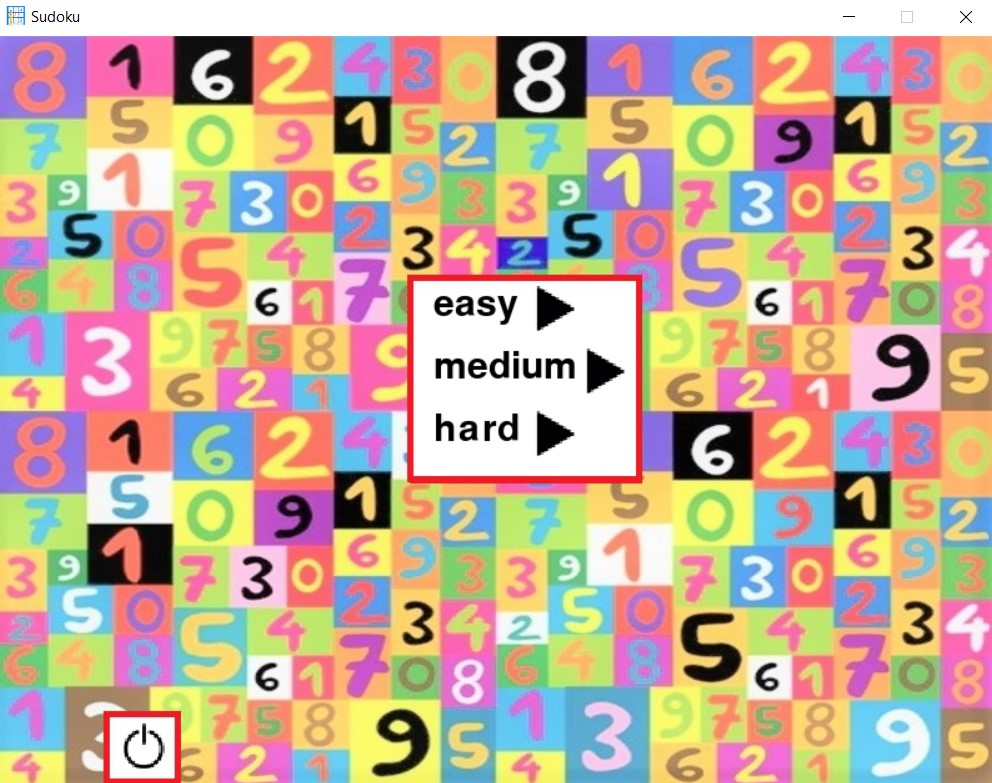
\includegraphics[width=0.8\linewidth]{3.jpg}
  \caption{Pagina secundara - alegerea nivelului}
  \label{fig:3rd}
\end{center}
\end{figure}

Diferenta intre cele trei niveluri este atat aspectul, cat si complexitatea de rezolvare. Primul nivel, cel mai usor este alcatuit din 2 x 2 regiuni si 4 x 4 celule care urmeaza sa fie completate. Nivelul al doilea, cel mediu contine 2 x 3 regiuni si 6 x 6 celule. Ultimul nivel, cel dificil vine cu varianta clasica de Sudoku, si anume 3 x 3 regiuni si 9 x 9 celule. Toate cele trei au completate in faza initiala un numar de celule, astfel conditionand utilizatorul sau, in cazul de fata, algoritmul care rezolva puzzle-ul.

\begin{figure}[!htb]
\minipage{0.32\textwidth}
  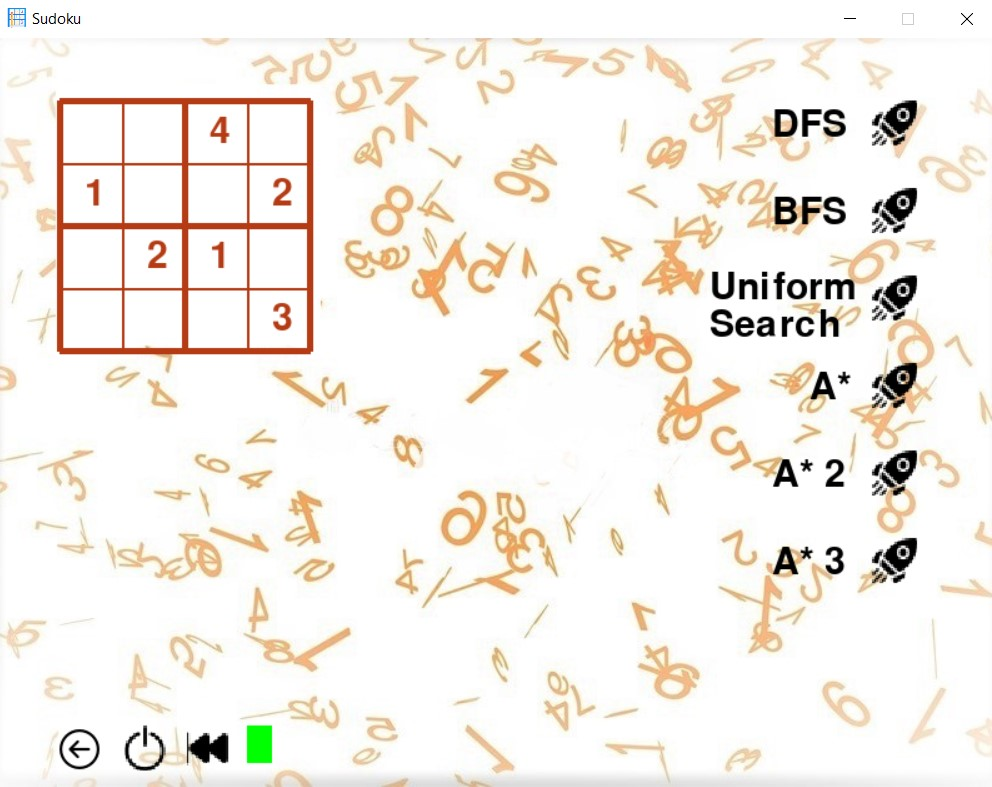
\includegraphics[width=\linewidth]{4.jpg}
  \caption{EASY}\label{fig: EASY}
\endminipage\hfill
\minipage{0.32\textwidth}
  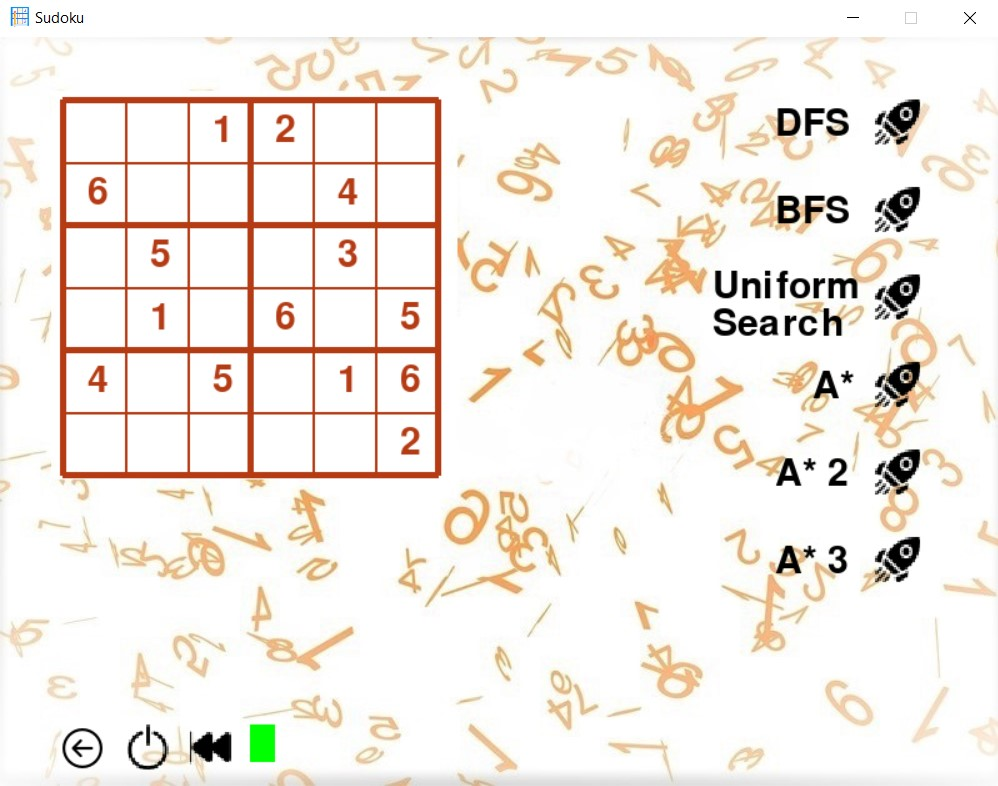
\includegraphics[width=\linewidth]{5.jpg}
  \caption{MEDIUM }\label{fig: MEDIUM}
\endminipage\hfill
\minipage{0.32\textwidth}%
  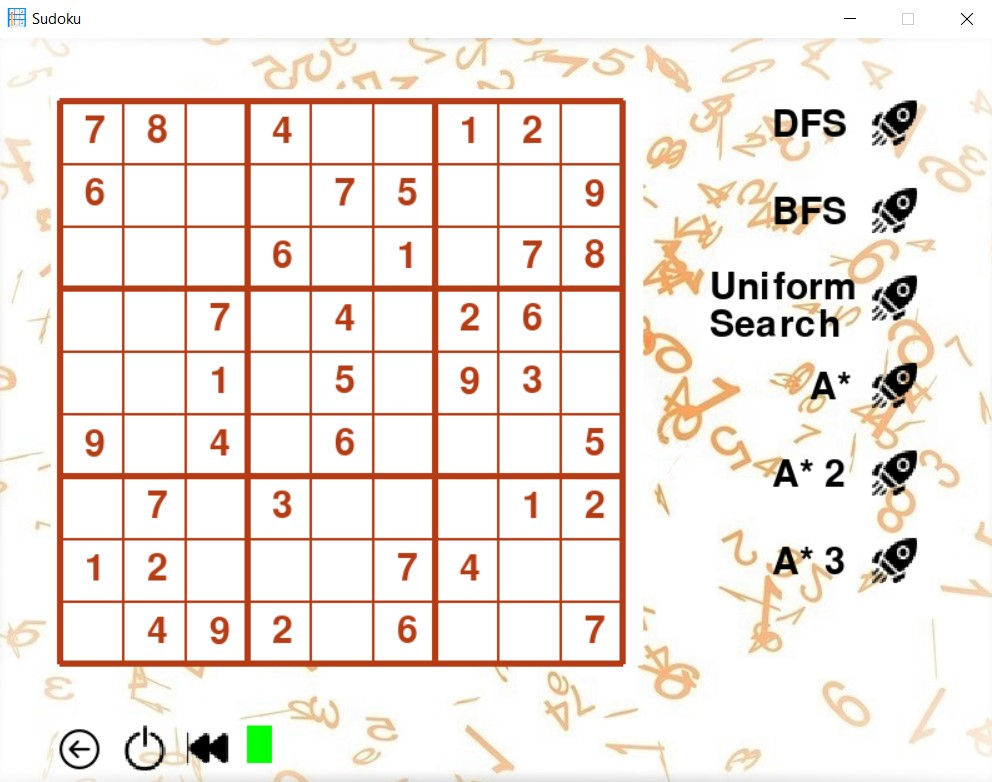
\includegraphics[width=\linewidth]{6.jpg}
  \caption{HARD}\label{fig: HARD}
\endminipage
\end{figure}

Fisierul util.py contine declarari de structuri de date, precum: stiva, coada sau coada de prioritati si functiile lor specifice.
\newline 
\\ \indent "Sudoku.py" este compus din metodele de rezolvare a jocului, acestea fiind descrise in capitolul 3.

\newpage
\section{ Metode de rezolvare}
\subsection{ DFS - Depth-first search}

\tab Incepem prin a seta startul ca fiind starea initiala a matricei de Sudoku corespunzatoare nivelului, initializam o lista cu pozitiile explorate de algoritm si o stiva cu starile reprezentate de matricea completata cu numerele care corespund pozitiilor libere din matrice. Adaugam starea de start in stiva. Cat timp stiva nu e goala, scoatem din stiva ultimul element adaugat. Il adaugam si in lista board\_frames pentru a ajuta la animatiile cu rezolvarea jocului si pentru a pastra toate schimbarile pe care le-a suferit tabla initiala. Verificam daca nu e rezolvat deja jocul - prin metoda isGoalState, adica daca nu mai exista nici o pozitie libera ramasa. In caz contrar gasim prima pozitie libera din matricea curenta. In functie de nivel, incercam sa gasim numerele care se potrivesc pe pozitia actuala. Daca gasim numere care se pot introduce pe poziita la care ne aflam, facem o copie a matricei unde adaugam numarul descoperit. Aceasta matrice urmeaza sa fie inclusa in stiva, iar pozitia alaturi de valoarea pe care am adaugat-o, in lista explored[]. La final daca s-a gasit solutia se returneaza - prin returneaza[].
\newline 
\\ \indent Spre deosebire de algoritmul general DFS, noi nu am mai verificat daca pozitia curenta cu numarul valid se gasesc deja in explored deoarece algoritmul se intoarce de cele mai multe ori in spate si unele locuri libere au doar o anumita valoare valida de completat, daca am verifica daca exista deja in explored cand ajunge la o pozitie deja parcursa dar golita nu ar mai putea continua si astfel nu va gasi rezolvarea corecta a jocului de Sudoku.

\subsection{ BFS - Breadth-first search}

\tab Incepem mai intai prin a seta startul ca fiind starea initiala a matricei de sudoku corespunzatoare nivelului, declaram o lista cu pozitiile explorate de algoritm si o coada cu starile reprezentate de matricea completata cu numerele care corespund pozitiilor libere din matrice. Adaugam starea de start in coada. Cat timp coada nu e goala, scoatem primul element din coada. Il adaugam si in lista board\_frames pentru a ajuta la animatiile cu rezolvarea jocului si pentru a pastra toate schimbarile pe care le-a suferit tabla initiala. Verificam daca nu e rezolvat deja jocul - prin metoda isGoalState, adica daca nu mai exista nici o pozitie libera ramasa. In caz contrar gasim prima pozitie libera din matricea curenta. In functie de nivel, incercam sa gasim numerele care se potrivesc pe pozitia curenta. Daca gasim numere care se pot introduce pe poziita respectiva, facem o copie a matricei curente unde adaugam numarul gasit si adaugam aceasta matrice in coada iar pozitia impreuna cu valoarea pe care am adaugat-o, in lista explored[]. La final daca s-a gasit solutie se returneaza solutia, altfel se returneaza[].
\newline 
\\ \indent Spre deosebire de algoritmul general BFS, nu se face verificarea daca pozitia curenta cu numarul valid se gasesc deja in explored deoarece algoritmul se intoarce de cele mai multe ori in spate si unele locuri libere au doar o anumita valoare valida de completat, daca am verifica existenta acesteia in explored, atunci cand ajunge la o pozitie deja parcursa dar golita sa nu mai poate continua si astfel nu va gasi rezolvarea corecta a jocului de sudoku.

\subsection{ UNIFORM SEARCH}

\tab Pentru acest algoritm, de asemenea, Incepem mai intai prin a seta startul ca fiind starea initiala a matricei de sudoku corespunzatoare nivelului. Diferenta consta in initializarea costului newcost cu 0, pe care il vom folosi la calcularea noului cost la trecerea pe o alta pozitie, initializam o lista cu pozitiile explorate de algoritm si o coada de prioritati cu starile reprezentate de matricea completata cu numerele care corespund pozitiilor libere din matrice. 
\newline
\\ \indent Adaugam si starea de start in coada impreuna cu costul 0 si prioritatea 0. Cat timp coada de prioritati nu e goala, scoatem primul element din coada, constituit din currentB reprezentand matricea pe care urmeaza sa facem verificari si costul. Adaugam currentB si in lista board\_frames pentru a ajuta la animatiile cu rezolvarea jocului de Sudoku si pentru a pastra toate schimbarile pe care le-a suferit tabla initiala. Verificam daca nu e rezolvat deja jocul, isGoalState, adica daca nu mai exista nici o pozitie libera ramasa. In caz contrar gasim prima pozitie libera din matricea curenta. 
\newline
\\ \indent In functie de dificultatea aleasa, incercam sa gasim numerele care s-ar potrivi pe pozitia curenta. Daca gasim numere care se pot introduce pe poziita respectiva, facem o copie a matricei curente unde adaugam numarul gasit pe pozitia curenta si adaugam aceasta matrice in coada impreuna cu noul cost si prioritatea acestuia, iar pozitia, impreuna cu valoarea pe care am adaugat-o, in lista explored[]. Calculam noul cost ca fiind costul precedent +1. La final daca s-a gasit solutia potrivita, aceasta se returneaza si costul rezultat in urma gasirii acesteia.

\subsection{A* }

\tab Initial, setam startul ca fiind starea initiala a matricei de sudoku corespunzatoare nivelului, initializam costul newcost cu 0, pe care il vom folosi la calcularea noului cost la trecerea pe o alta pozitie, folosim o lista cu pozitiile explorate de algoritm si o coada de prioritati cu starile reprezentate de matricea completata cu numerele care corespund pozitiilor libere din matrice. 
\newline
\\ \indent Adaugam si starea de start in coada impreuna cu costul 0 si prioritatea data de heuristica folosita. Cat timp coada de prioritati nu e goala, scoatem primul element din coada, constituit din currentB reprezentand matricea pe care urmeaza sa facem verificari si costul. Adaugam currentB si in lista board\_frames pentru a ajuta la animatiile cu rezolvarea jocului si pentru a pastra toate schimbarile pe care le-a suferit tabla initiala. Verificam daca nu e rezolvat deja jocul, isGoalState, adica daca nu mai exista nici o pozitie libera ramasa. In caz contrar gasim prima pozitie libera din matricea curenta. 
\newline
\\ \indent In functie de nivel, incercam sa gasim numerele care s-ar potrivi pe pozitia curenta. Daca gasim numere care se pot introduce pe poziita respectiva, facem o copie a matricei curente unde adaugam numarul gasit pe pozitia curenta si adaugam aceasta matrice in coada impreuna cu noul cost si prioritatea acestuia in coada, iar pozitia, impreuna cu valoarea pe care am adaugat-o, in lista explored[]. Calculam noul cost ca fiind costul precedent +1 + costul dat de heuristica folosita. La final daca s-a gasit solutie se returneaza solutia si costul rezultat in urma gasirii acesteia.

\subsection{HEURISTIC }

\tab NULL HEURISTIC - Aceasta heuristica este triviala, returneaza doar 0 intotdeauna. \newline 
\\ \indent HEURISTIC 2 - Aceasta heuristica returneaza cate pozitii libere mai sunt ramase in tabla jocului. \newline 
\\ \indent HEURISTIC 3 - Aceasta heuristica returneaza cate zone sunt ramase libere in tabla jocului. 

\section{ Asemanari si diferente}

\tab BFS vs DFS:
\newline 
\\ \indent BFS foloseste structura de tip coada pentru a gasi cea mai scurta cale folosind varfurile, spre deosebire de DFS, care foloseste stiva, unde e posibil sa fie utilizate mai multe varfuri pentru a ajunge la destinatie. Ambele sunt potrivite pentru jocuri de tip puzzle. Complexitatea este identica O(V + E). Legat de parcurgere, BFS viziteaza fratii nodului inaintea copiilor, iar DFS viziteaza copiii inaintea fratilor. 
\newline 
\\ \indent Uniform-search vs A*
\newline 
\\ \indent Uniform-search nu foloseste niciun tip de informatie despre final cautarea este in toate directiile. Poate fi vazuta ca si o functie f(n) = g(n), unde g - costul. A* foloseste heuristica pentru a estima cat de aproape de rezultatul final se afla. Ambele metode au lista de noduri expandate, dar A* incearca sa minimizeze lista aceasta prin - path cost + heuristic function -.

\newpage
\section{ Bibliografie}

\tab https://newbedev.com/what-is-the-difference-between-uniform-cost-search-and-best-first-search-methods
\newline 
\\ \indent https://www.geeksforgeeks.org/difference-between-bfs-and-dfs/?ref=lbp
\newline 
\\ \indent https://www.youtube.com/watch?v=G8MYGDf\_9ho\&t=970s
\newline 
\\ \indent https://www.youtube.com/watch?v=lK4N8E6uNr4\&t=267s
\newline 
\\ \indent https://latex-tutorial.com/

\end{document}